\documentclass[11pt]{scrartcl}
\usepackage{amsmath}
\usepackage{amssymb}
\usepackage[ngerman]{babel}
\usepackage[pdftex]{graphicx}
\usepackage{epstopdf}
\usepackage{hyperref}
\usepackage[utf8]{inputenc}
\usepackage{verbatim}

\graphicspath{{./}{plots/}}

\title{VDVC Survey}
\author{Patrik Schönfeldt}
\date{\today}

\begin{document}
\maketitle

\section{Beschreibung der Stichprobe}
Der erste Teil der VDVC-Umfrage (künftig: \emph{2013}) wurde über insgesamt 14 Tage
vom 23. Dezember 2013 bis zum 6. Januar 2014 durchgeführt.
1417 Personen haben diesen Teil abgeschlossen.
Die Fortsetzung (künftig: \emph{2014}) wurde
den kompletten Dezember 2014 durchgefüht,
die Zahl der komplett abgeschlossenen Fragebögen beträgt 3359.
In beiden Fällen wurde bei den Communities \emph{For Uncut!},
\emph{Stigma-Videospiele/VDVC} und \emph{World of Players} für die Umfrage
geworben.
2014 hat insbesondere einen Hinweis bei \emph{GameStar} und \emph{GamePro}
die Reichweite nochmals erhöht.

Da der befragte Personenkreis nicht als konstant angenommen werden kann,
muss für die Feststellung von Trends auf Veränderungen in der Stichprobe
Rücksicht genommen werden.
Die folgenden Untersuchungen sollen diese Vergleichbarkeit herstellen
und auch Aufschluss über die Repräsentativität der Umfrage geben.

\subsection{Altersstruktur}

\begin{figure}[htbp]
	\centering
	\includegraphics[width=0.48\linewidth]{2013/alter}\hfill
	\includegraphics[width=0.48\linewidth]{2014/alter}
	\caption[Altersstruktur]
	{Die Altersstruktur des Teilnahmefelds folgt in beiden Jahren einem
	ähnlichen Muster.
	Jeweils gibt es kaum Teilnehmer unter 15 Jahren,
	ab 20 Jahren erreicht die Verteilung ein Plateau.
	Zwischen 40 und 50 Jahren sind nur wenige,
	noch älter kaum noch Teilnehmer.}
	\label{fig:alter}
\end{figure}

\subsection{Geschlechter}

\begin{figure}[htbp]
	\centering
	\includegraphics[width=0.48\linewidth]{2013/geschlecht-rel}\hfill
	\includegraphics[width=0.48\linewidth]{2014/geschlecht-rel}
	\caption{Geschlechter}
	\label{fig:geschlecht}
\end{figure}

\clearpage
\bibliography{VDVC-Survey}{}
\bibliographystyle{alpha}

\end{document}
